\section{Baseline Architecture}

    \begin{figure}
        \begin{center}
            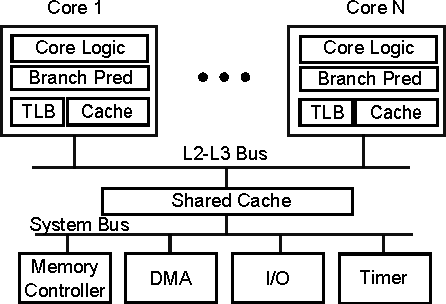
\includegraphics[width=3.5in]{figs/baseline.pdf}
            \caption{The timing-channel vulnerable baseline architecture.}
            \label{fig:baseline}
        \end{center}
    \end{figure}

    Figure \ref{fig:baseline} shows the baseline architecture which is later extended to 
    include timing channel protection. The architecture has multiple cores, 
    each with a branch predictor, one or more private caches, a TLB, and the 
    core logic. Each processor is connected to a shared cache through an 
    on-chip network. The multicore processor is connected to the main memory 
    and a DMA module through the system bus. 
